\chapter{制約充足問題} \label{chap:CSP}
制約充足問題(Constraint Satisfaction Problem, CSP)は, 計算量理論において重要な問題の一つであり, PCP定理の証明においても中心的な役割を果たす.

\section{制約充足問題の定義}
制約充足問題とは端的に言えば連立方程式の解の存在性判定を問う判定問題である.

\begin{definition}{制約充足問題}{CSP}
\emph{制約充足問題(CSP)}とは次の要素からなる組$\varphi = (X,\Sigma,\calI,\calC)$をインスタンスとする判定問題である:
\begin{itemize}
  \item \emph{アルファベット}: 有限集合$\Sigma$.
  \item \emph{変数列}: $X=(\varx_1,\dots,\varx_n)$.
  \item 制約の引数の列: $\calI=(I_1,\dots,I_m)$. ここで, 各$I_i$は $I_i\ne\emptyset$ かつ $I_i\subseteq [n]$を満たす.
  \item \emph{制約の列}: $\calC=(c_I)_{I\in\calI}$. ここで, 各$c_I$は$c_I \subseteq \Sigma^{\abs{I}}$を満たす.
\end{itemize}
各$\varx\in X$を\emph{変数}, 各$c_I\in\calC$を\emph{制約}という.

入力$(X,\Sigma,\calI,\calC)$は,
ある変数への割り当て$a \colon X \to \Sigma$が存在して, 任意の$I=\{i_1,\dots,i_k\}\in\calI$ (ただし$i_1<\dots<i_k$)について,
\begin{align*}
  (a(\varx_{i_1}),\dots,a(\varx_{i_k})) \in c_I
\end{align*}
であるとき, かつその時に限りYesインスタンスである.
また, 変数の個数と制約の個数の和$n+m$を$\varphi$の\emph{サイズ}といい, $\size(\varphi)$と表す.

全ての$i\in[m]$について$\abs{I_i}\le q$であるとき, このCSPは\emph{$q$-CSP}という.

また, 固定した割り当て$a \colon X\to \Sigma$に対する$\varphi$の\emph{不満足値}を
\begin{align*}
  \UNSAT(a;\varphi) = \Pr_{\qty{i_1,\dots,i_k}\sim\calI}\qty[(a(\varx_{i_1}),\dots,a(\varx_{i_k})) \not\in c_I]
\end{align*}
とする. ここで$I\sim\calI$は$I$が$\calI$から一様ランダムに選ばれたことを意味する.
さらに, 全ての割り当てに関して不満足値の最小値
\begin{align*}
  \UNSAT(\varphi) = \min_{a\colon X\to\Sigma} \UNSAT(a;\varphi)
\end{align*}
を$\varphi$の\emph{不満足値}という.
\end{definition}

各制約$c_I\in \calC$は, その制約が充足される割り当ての集合を表す.
例えば$c_I = \Sigma^{\abs{I}}$であるならば, 任意の割り当てに対して$c_I$は充足されるし,
$c_I = \emptyset$であるならば, どの割り当ても$c_I$を充足しない.

\begin{example}{グラフ彩色問題}{graph-coloring-problem-CSP}
  グラフ彩色問題(\cref{ex:graph-coloring-problem})は$2$-CSPである.
  実際, グラフ$G=(V,E)$に対して
  \begin{itemize}
    \item 変数列を$X=V$とする.
    \item アルファベットを$\Sigma=[k]$とする.
    \item 辺の順序が固定された辺集合$E=\qty{e_1,\dots,e_m}$に対し, $\calI = (e_1,\dots,e_m)$とする.
    \item 各制約$c_e$は各辺$e=\{u,v\}\in E$に付随していて,
    \begin{align*}
      (a_u,a_v) \in c_e \iff a_u\ne a_v
    \end{align*}
  と定義する.
  \end{itemize}
  このとき, グラフ$G$が$k$-彩色可能であることと, このCSPがYesインスタンスであることは同値である.
\end{example}

\begin{example}{二次方程式系の充足可能性判定問題}{ThreeQuadEQ-3-CSP}
  \cref{thm:ThreeQuadEQ-NP-complete}で定義した判定問題$\ThreeQuadEQ$は$3$-CSPである.
  $\ThreeQuadEQ$のインスタンス$f_1,\dots,f_m\colon\F_2^n\to\F_2$に対し,
  変数を$x_1,\dots,x_n$とし, $f_i(x)=0$という制約を考えると, 各$f_i$の出力は高々三つの変数の値にのみ依存するため, これは$3$-CSPである.
\end{example}

以後は, \cref{ex:ThreeQuadEQ-3-CSP}のように, $k$-CSPの定義を与える際は, $calI$や$calC$を明示せずに全ての変数と制約を記述することによって与えることもある.


\subsection{PCPとの関係}
ランダムシード長$r=r(n)$かつクエリ数$q=O(1)$のPCP検証者は$\Sigma=\{0,1\}$の場合の$q$-CSPによって表現でき, 逆に$q$-CSPはPCP検証者として表現できる.
実際, $q$クエリのPCP検証者$V^\pi(x)$を考えよう.
証明の長さを$\abs{\pi}=\ell$とする.
入力$x$とランダムシード$s$を固定したときの$V^\pi(x;s)$が
証明中の読み込む文字のインデックスの集合を$I_s\subseteq[\ell]$とする (ここで$\abs{I_s}\le q$).
このとき, $V^\pi(x;s)$は$\binset^{I_s}$を$\binset$に写す関数を定める.
この関数を制約$c_s$とみなすことで, 検証者$V^\pi(x)$は$q$-CSPのインスタンスとして表現できる.
このとき, $q$-CSPのインスタンスの変数集合は証明$\pi$に対応する.
もし$x\in L$であるならば, 確率$1$で$V^\pi(x)=1$となるような$\pi$が存在する.
つまり, 全てのランダムシード$s$に対して$V^\pi(x;s)=1$となるような$\pi$が存在するため,
先ほど構成した$q$-CSPのインスタンスはYesインスタンスである.
逆に$x\not\in L$であるならば, 全ての$\pi$に対して確率$1/3$以上で$V^\pi(x)=0$となる.
これは, $q$-CSPインスタンスに対して, 全ての割り当てを考えても, 全体の制約のうち少なくとも$1/3$の割合は充足されない(すなわち, $\UNSAT$の値が$1/3$以上となる)ことを意味する.


\begin{table}[htbp]
  \centering
  \begin{tabular}{|c|c|}
    \hline
    PCP検証者 & $q$-CSP \\
    \hline
    PCP $\pi$ & 割り当て \\
    \hline
    ランダムネスを固定した時の判定 & CSPの制約 \\
    \hline
    PCP$\pi$を拒否する確率 & 割り当ての不満足値 $\UNSAT(\pi)$ \\
    \hline
  \end{tabular}
  \caption{PCPとCSPの対応関係}
  \label{table:pcp-csp-correspondence}
\end{table}

この対応関係に基づいて, PCP定理をCSPを用いた言葉で表すことができる.

\begin{theorem}{PCP定理のCSP版}{PCP-CSP-theorem}
  ある関数$K(s)=s^{O(1)}$, 定数$c\in\Nat$, $q\in\Nat$, $\alpha>0$, および
  次の性質を満たす多項式時間決定的アルゴリズムが存在する:
  $\ThreeQuadEQ$のインスタンス$\varphi_0=(f_k)$を入力として受け取り, $q$-CSPのインスタンス$\varphi=(X,\Sigma,\calI,\calC)$を出力する.
  このインスタンス$\varphi$は, 与えられた$\varphi_0$のサイズが$s=\size(\varphi_0)$であるとき, $\size(\varphi)=K(s)$, $\abs{\Sigma}=c$となる.
  さらにこのインスタンス$\varphi$は
  \begin{itemize}
  \item 入力$\varphi_0$が$\UNSAT(\varphi_0)=0$である(すなわち$\ThreeQuadEQ$のYesインスタンスである)とき, $\UNSAT(\varphi) = 0$となる.
  \item 入力$\varphi_0$が$\UNSAT(\varphi_0)>0$である(すなわち$\ThreeQuadEQ$のNoインスタンスである)とき, $\UNSAT(\varphi) \ge \alpha$となる.
  \end{itemize}
\end{theorem}

\begin{remark}{}{}
  一般に$m$個の制約からなるCSPのインスタンス$\varphi_0$がNoインスタンスであることは$\UNSAT(\varphi_0)\ge \frac{1}{m}$と同値である.
  ところが\cref{thm:PCP-CSP-theorem}では, 変換によって得られるCSPのインスタンス$\varphi$のサイズが元のCSPのインスタンス$\varphi_0$のサイズ$s$に\emph{よらない定数になる}点が重要である.
\end{remark}

PCP検証者の構成とCSPの変換が同値であることを証明する.

\begin{lemma}{PCP検証者とCSPの変換の同値性}{equivalence-of-pcp-verifier-and-csp-transformation}
  \cref{thm:PCP-CSP-theorem}と\cref{thm:QuadEQ-PCP-verifier}は同値である.
\end{lemma}
\begin{proof}
  それぞれの方向を別々に証明する.

  \emph{\cref{thm:PCP-CSP-theorem}$\Rightarrow$\cref{thm:QuadEQ-PCP-verifier}の証明.}
  ある$r=O(\log n)$, $q'=O(1)$に対して, $\ThreeQuadEQ$に対するシード長$r$, クエリ回数$q'$のPCP検証者$V^\pi$を構成する.
  検証者はまず入力として$\ThreeQuadEQ$のインスタンス$\varphi_0=(f_k)$を受け取り, \cref{thm:PCP-CSP-theorem}のアルゴリズムを用いて$q$-CSPのインスタンス$\varphi$を計算する.
  また, 証拠$\pi$をこの$q$-CSPのインスタンス$\varphi$の割り当てとして解釈し,
  PCP検証者$V^\pi(\varphi_0)$は以下の操作を十分大きな定数回繰り返す: 一様ランダムに$\varphi$の制約$c_i$を選択し, その制約に含まれる変数に対する割り当て$\pi$の値を読み込み, この制約$c_i$が読み込んだ割り当てによって充足\emph{されない}ならば$0$を出力し終了する. 何度も繰り返した末に終了しなかったのであれば, $1$を出力して終了する.
  この検証者は繰り返しの回数が$O(1)$であり, それぞれの繰り返しにおいては高々$q$個の変数の値を読み込むため, クエリ回数は$q'=O(q)=O(1)$となる. なお, ここでアルファベットサイズ$c$が定数であるため, 全体で読み込む証明のビット数は$q'\cdot\ceil{\log_2 c}=O(1)$ことに留意する.
  また, ランダムシードはランダムな制約を選ぶために使われてるため, その長さは$O(\log K(\size(\varphi_0)) = O(\log \size(\varphi_0))$となる.

  もし$\varphi_0$がYesインスタンスならば, $\varphi$もYesインスタンスであるため, $\pi$をその充足割り当てとすれば, 全ての制約$c_i$が充足されるため, (制約の選び方のランダムネスに関して)確率$1$で$V^\pi(\varphi_0)=1$となる.
  もし$\varphi_0$がNoインスタンスならば, $\UNSAT(\varphi) \ge \alpha$である. 従って, 任意の割り当て$\pi$に対して, 一様ランダムな制約$c_i$が充足される確率は高々$1-\alpha$である.
  よって, この操作を$\ceil{10/\alpha}=O(1)$回繰り返すと, 少なくとも確率$1/3$で充足されない制約が一度以上選ばれ, 検証者は$0$を出力する.


  \emph{\cref{thm:QuadEQ-PCP-verifier}$\Rightarrow$\cref{thm:PCP-CSP-theorem}の証明.}
  仮定より, $\ThreeQuadEQ$に対する, ランダムシード長$r=O(\log n)$, クエリ回数$q=O(1)$のPCP検証者$V^\pi$が存在する. アルゴリズム$A$は, 入力$\varphi_0=(f_k)$に対して, 全てのランダムシード$s\in \binset^r$を列挙して, それぞれに対して「$V^\pi(\varphi_0;s)=1$」という制約を加えて得られるCSPを出力する. 各$V^\pi(\varphi_0;s)$は, $\pi$を変数とみなしたとき, 高々$q$個の変数の値を読み込むため, $(c_s)_{s\in\binset^r}$は$2^r=n^{O(1)}$個の制約からなる$q$-CSPとなる.
  なお, $V^\pi$は多項式時間アルゴリズムなので, $A$も多項式時間アルゴリズムである.
\end{proof}

従って, 以降は\cref{thm:PCP-CSP-theorem}の証明に注力する.

\subsection{制約グラフ}
PCP定理の証明, すなわち\cref{thm:PCP-CSP-theorem}の証明は, まず$3$-CSPの特殊ケースである$\ThreeQuadEQ$を$2$-CSPに変換し, この$2$-CSPに対して様々な変換を繰り返し施すことによって得られる.
$2$-CSPは各制約が高々一つの変数への割り当てのみに依存するものであるため, その制約をグラフとして記述することができる.
このような$2$-CSPのグラフ表現を\emph{制約グラフ}という.

\begin{definition}{制約グラフ}{constraint-graph}
  2-CSPのインスタンス$\varphi=(X,\Sigma,\calI,\calC)$に対し, 以下で定まる組$G=\ip{(V,E),\Sigma,\calC'}$を\emph{制約グラフ}という\footnote{制約グラフの表記に用いる括弧は形式的には本来$((V,E),\Sigma,\calC')$のようにすべきだが, 可読性のためあえて外側の括弧を$\ip{\cdot}$としている.}:
  \begin{itemize}
    \item $(V,E)$はグラフである. ただし頂点集合は$V=X$であり, 辺集合は$E=\calI$である. なお, ここで考えるグラフは多重辺や自己ループを持ちうるもの\footnote{具体的には$E$は多重集合であり, 自己ループに対応する辺は$\{u\}$と表す. 詳細は\cref{def:multigraph}を参照.}とし, 特に$\abs{I_i}=1$の場合は対応する辺は自己ループとする.
    \item アルファベット$\Sigma$.
    \item 制約の列$\calC'=(c'_e)_{e\in E}$は, $\abs{e}=2$ならば$c'_e=c_e$とし, $\abs{e}=1$ならば$c'_e=\qty{ (u,u) \in \Sigma^2 \colon u\in e }$とする. これにより, 全ての$c'_e$は$\Sigma^2$の部分集合となる.
  \end{itemize}

  制約グラフ$G=\ip{(V,E),\Sigma,\calC}$および割り当て$a\colon V\to \Sigma$に対して, その\emph{不満足値}を
  \begin{align*}
    \UNSAT(a;G) = \Pr_{e\sim E}[a(e) \not\in c_e]
  \end{align*}
  と定義し (ここで$e=\{u,v\}$ ($u<v$)に対して$a(e)=(a(u),a(v))\in\Sigma^2$とする), $G$の不満足値を
  \begin{align*}
    \UNSAT(G) = \min_{a\in\Sigma^V} \UNSAT(a;G)
  \end{align*}
  と定義する.

  制約グラフ$G=\ip{(V,E),\Sigma,\calC}$に対して, その\emph{サイズ}を
  \begin{align*}
    \size(G) = \abs{V} + \abs{E}
  \end{align*}
  と定義する.
\end{definition}

\begin{remark}{入力長とサイズの関係}{input-length-and-size-relation}
  本講義で考える制約グラフのアルファベットサイズ$\abs{\Sigma}$は常に定数, すなわち$\abs{V}$や$\abs{E}$に依存しない値であるとする.
  この仮定の下, 制約グラフ$G=\ip{(V,E),\Sigma,\calC}$を指定するために必要なビット数を考える.
  グラフ$(V,E)$は隣接行列で表現すると$\abs{V}^2$ビットで表現できる.
  各辺$e\in E$に付随する制約$c'_e\subseteq\Sigma^2$は, 各$(a,b)\in\Sigma^2$について$(a,b)\in c'_e$かどうかを表すビットを$(a,b)$について並べれば良いため, 全部で$\abs{E}\cdot\abs{\Sigma}^2$ビットで表現できる.
  よって, 制約グラフ$G$は$\abs{V}^2+\abs{E}\cdot\abs{\Sigma}^2 = O(\size(G)^2)$ビットで表現できる.
  このことから, 制約グラフを入力として受け取るアルゴリズムが多項式時間かどうかを議論する際は, その時間計算量が$\size(G)$に関して多項式かどうかを議論すれば良いことになる.
\end{remark}

制約グラフは2-CSPを表現するためのものであるが, 一般の$k$-CSPもまた制約グラフとして表現することができる.
\begin{lemma}{k-CSPの制約グラフ表現}{k-CSP-constraint-graph-representation}
  任意の$k\in\Nat$に対し, ある定数$c>0$および多項式時間アルゴリズム$A$が存在して次が成り立つ:
  $k$-CSPのインスタンス$\varphi=(X,\Sigma,\calI,\calC)$を入力として受け取り, 以下を満たす制約グラフ$G=\ip{(V,E),\Sigma^k,\calC'}$を出力する.
  \begin{itemize}
    \item $\size(G) \le ck\cdot(\abs{X}+\abs{\calI})$
    \item $\UNSAT(\varphi)=0$ならば$\UNSAT(G)=0$.
    \item $\UNSAT(\varphi)>0$ならば$\UNSAT(G) \ge \frac{1}{k}\cdot \UNSAT(\varphi)$.
  \end{itemize}
\end{lemma}
\begin{proof}
  入力として与えられた$k$-CSPの変数集合$X=\qty{\varx_1,\dots,\varx_n}$および制約集合$\calC=(c_I)_{I\in\calI}$に対し,
  新たに構成する制約グラフは次のような構造を持つ:
  $\varphi$の各変数$\varx_i$に対し頂点$x_i$を用意し, 各制約$c_I$ ($I\in\calI$)に対し頂点$y_I$を用意する.
  変数$\varx_i$が制約$c_I$に含まれる, すなわち$\varx_i\in I$ならば, 二頂点$x_i$と$y_I$の間に辺を引いて得られる二部グラフを$(V,E)$とする.
  簡単のため, 以下では各$I\in\calI$に対して$\abs{I}=k$とする (そうでない制約が存在するならば, そのような各制約は同じ変数を複数回読み込むことを許し, 対応する辺は多重辺とすることで, 読み込み回数をちょうど$k$にする).
  この二部グラフは, 各$y_i$の次数はちょうど$k$であり, サイズは($k$のみに依存する)定数倍で抑えられる.

  \begin{figure}[ht]
    \centering
    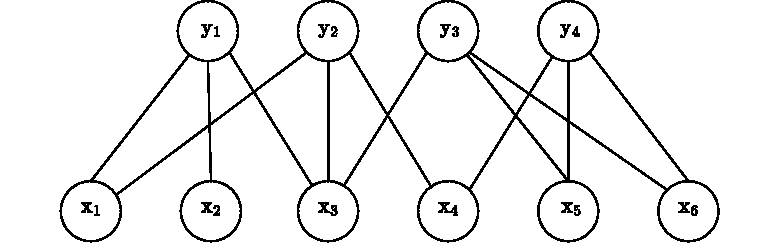
\includegraphics[width=0.8\textwidth]{images/k-to-two.pdf}
    \caption{制約グラフの構成例. 例えば, 変数$\vary_1$に対応する制約は変数$\varx_1,\varx_2,\varx_3$に依存している. \label{fig:k-to-two}}
  \end{figure}

  新たな制約グラフのアルファベットは$\Sigma^k$とする.
  各辺$e=\{x_i,y_I\}$に対応する制約$c'_e$は, 割り当て$x_i\leftarrow \vec{\sigma}=(\sigma_1,\dots,\sigma_k)\in\Sigma^k$, $y_I\leftarrow \vec{\tau}=(\tau_1,\dots,\tau_k)\in\Sigma^k$が次の条件を満たすとき, かつその時に限り充足される: $y_I$の隣接頂点を$x_{i_1},\dots,x_{i_k}$ ($i_1<\dots<i_k$)としたとき,
  \begin{itemize}
    \item 部分割り当て$(\varx_{i_1}\leftarrow \tau_1,\dots,\varx_{i_k}\leftarrow \tau_k)$が$c_I$を充足する.
    \item $\tau_i = \sigma_1$
  \end{itemize}
  ここでは, $x_i$への割り当てのうち, $\sigma_2,\dots,\sigma_k$は無視されていることに留意されたい.

  \begin{figure}[ht]
    \centering
    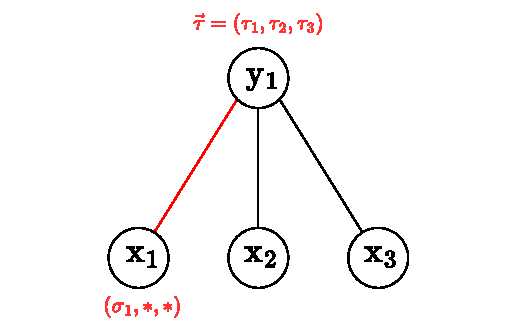
\includegraphics[width=0.6\textwidth]{images/k-to-two2.pdf}
    \caption{割り当ての例. ここでは, $(\tau_1,\tau_2,\tau_3)$が$\vary_1$に対する制約を充足し, さらに$\sigma_j=\tau_j$ ($j=1,2,3$)であれば, 辺$\{y_1,x_j\}$に対応する制約グラフの制約が満たされる. \label{fig:k-to-two2}}
  \end{figure}

  元の$k$-CSPのインスタンス$\varphi$が充足可能, すなわち$\UNSAT(\varphi)=0$ならば, その充足割り当て$a\colon X \to \Sigma$に対し, 
  制約グラフ$G$の割り当て$a'\colon V\to \Sigma^k$を
  \begin{align*}
    & a'(x_i) = (a(\varx_i),\underbrace{\ast,\dots,\ast}_{k-1}) \quad (i\in[n]), \\
    & a'(y_I) = \qty(a(\varx_{i_1}),\dots,a(\varx_{i_k}),\sigma_1) \quad (I=\qty{i_1,\dots,i_k}\in\calI).
  \end{align*}
  と定める ($\ast$は$\Sigma$の任意の元でよい). この割り当て$a'$は$G$の全ての制約を満たすため, $\UNSAT(G)=0$である.

  逆に, $G$の任意の割り当て$a'\colon V\to \Sigma^k$に対し, $\varphi$の割り当て$a\colon X\to \Sigma$を
  \begin{align*}
    a(\varx_i) = a'(x_i)_1 \quad (i\in[n])
  \end{align*}
  と定める.
  割り当て$a'$が頂点$y_I$に接続する全ての辺$\{x_i,y_I\}$ ($\forall i\in I$)に対応する$G$の制約を充足するならば,
  割り当て$a$は制約$c_I$を満たす.
  対偶をとると, $a$が$c_I$を満たさないならば, $a'$は少なくとも1つの辺$\qty{\{x_i,y_I\}}_{i\in I}$に対応する制約が充足されない.
  すなわち$\UNSAT(a';G) \ge \frac{1}{k}\cdot \UNSAT(a;\varphi)$である.
  従って, 割り当て$a'$を$\UNSAT(a';G)=\UNSAT(G)$となるように選ぶと
  \begin{align*}
    \UNSAT(G) = \UNSAT(a';G) \ge \frac{\UNSAT(a;\varphi)}{k}  \ge \frac{\UNSAT(\varphi)}{k}
  \end{align*}
  より, 主張を得る.
  
\end{proof}

\section{多重グラフの導入とエクスパンダーグラフ}

以後, 制約グラフに関する様々な操作をしていく上で多重グラフのフォーマルな定義を与えておく.

\begin{definition}{多重グラフ}{multigraph}
有限集合$V$と多重集合$E$の組$(V,E)$を\emph{多重グラフ}という.
ここで$E$は$V\cup \binom{V}{2}$の元から構成される多重集合であり, $e\in E$は$\abs{e}=1$ならば\emph{自己ループ}であるという.

二頂点$u,v\in V$の間の\emph{重み}を
\begin{align*}
  w(u,v) = \abs{\qty{e\in E \colon e = \{u,v\}}}
\end{align*}
と定義し, 頂点$u$の\emph{次数}を
\begin{align*}
  \deg(u) = \sum_{v\in V} w(u,v)
\end{align*}
と定義する.\footnote{自己ループの次数への寄与は$1$であることに留意されたい (文脈によってはこの寄与が$1$である場合もある).} また, $W=(w(u,v))_{u,v\in V}$を\emph{重み行列}と呼び, 
$P(u,v):=\frac{w(u,v)}{\deg(u)}$で定まる行列$P\in[0,1]^{V\times V}$を\emph{遷移確率行列}という.

\end{definition}

グラフの次数を並べたベクトル$d=(\deg(v))_{v\in V}\in \Real^V$を\emph{次数ベクトル}という.
次数ベクトルは
\begin{align*}
  d = W\allone
\end{align*}
で与えられる.
グラフ$G$が自己ループを含まない場合は握手補題が成り立つため$\sum_{u\in V}\deg(u) = 2\abs{E}$が成り立つが, そうでない場合は次数の総和は自己ループを一度ずつしかカウントしないため, 自己ループの個数を$\ell$とすると
\begin{align}
  \sum_{u\in V} \deg(u) = 2\abs{E} - \ell \le 2\abs{E} \label{eq:hand_shake_multigraph}
\end{align}
が成り立つ.


以下に正則グラフとエクスパンダーグラフの定義を述べる.

\begin{definition}{正則性とエクスパンダー性}{regularity-and-expander-graph}
  $n$頂点の多重グラフ$G=(V,E)$の全ての頂点の次数が$d$に等しいとき, $G$は\emph{$d$-正則}であるという.

  また, 遷移確率行列$P$の固有値$1=\lambda_1\ge \lambda_2\ge \cdots \ge \lambda_n \ge -1$が
  \begin{align*}
    \lambda(P):=\max\{\abs{\lambda_2}, \abs{\lambda_n}\} \le \lambda
  \end{align*}
  を満たすとき, $G$は\emph{$\lambda$-エクスパンダー}であるという.
\end{definition}

多重グラフ$G$が正則ならば$P$は対称行列となるため実固有値を持つことが直ちに従うが, 一般の場合でも実固有値を持つことが示せる.
さらに, Gershgorinの定理からそれらの固有値の絶対値は$1$以下であることが従う.
また, 全成分$1$のベクトル$\allone$は$P$の固有値$1$に対する固有ベクトルとなるため, $\lambda_1=1$である.

\begin{exercise}{}{}
  任意の多重グラフ$G$の遷移確率行列$P$は実固有値を持つことを示せ.
\end{exercise}

第一固有値$1$の多重度はグラフの連結成分の個数に等しいことが知られている.
ここではその特殊ケースである以下の事実を用いる.

\begin{proposition}{}{}
  多重グラフ$G$が連結であるならば, 遷移確率行列$P$の固有値$1$の多重度は$1$, すなわち$\lambda_2<1$である.
\end{proposition}

\subsection{正則エクスパンダーの性質}

この節では正則かつエクスパンダー性を持つ単純グラフの性質は同様に
多重グラフに対しても成り立つことを確認する.
特に, 正則性より遷移確率行列$P$は対称となることに留意されたい.

\begin{lemma}{エクスパンダー混交補題}{expander-mixing-lemma}
  連結な頂点数$n$の多重グラフ$G$が$d$-正則かつ$\lambda$-エクスパンダーであるとする.
  二つの頂点部分集合$S,T\subseteq V$に対して
  \begin{align*}
    W(S,T) = \sum_{u \in S, v\in T} w(u,v)
  \end{align*}
  とすると, 任意の$S,T\subseteq V$に対して
  \begin{align*}
    \abs{ W(S,T) - \frac{d}{n}\abs{S}\abs{T} } \le \frac{\lambda d}{n} \sqrt{\abs{S}\abs{T}\abs{V\setminus S}\abs{V\setminus T}}
  \end{align*}
  が成り立つ. 特に, $\abs{S}\le n/2$を満たす任意の$S\subseteq V$に対して
  \begin{align*}
    W(S,V\setminus S) \ge (1-\lambda)\frac{d\abs{S}}{2}
  \end{align*}
  が成り立つ.
\end{lemma}

\begin{remark}{直感的な意味}{intuitive-meaning-of-expander-mixing-lemma}
  簡単のため自己ループを持たないグラフを考える.
  このグラフが$n$頂点$d$-正則ならば全部で$nd/2$本の辺を持つ.
  全部で$\binom{n}{2}\approx n^2/2$個の頂点対があるため, 辺密度は$d/n$である.
  さて, グラフの辺が$\binom{V}{2}$に「均一に」散らばっていると仮定すると, 任意に固定した頂点部分集合$S,T\subseteq V$に対してその間をまたがる辺の本数$W(S,T)$はおよそ$(d/n)\cdot \abs{S}\abs{T}$であることが期待される.
  グラフ$G$がエクスパンダー性を持つ場合, この期待値からのずれの上からの評価を与えるのがエクスパンダー混交補題である.
\end{remark}

\begin{proof}
  「特に, ...」の部分は前半の主張に$T=V\setminus S$を代入して$\abs{V\setminus S}\ge n/2$を用いれば示せるので, 前半の主張を証明する.


  全成分$1$の行列$J \in \Real^{V\times V}$に対し, $M:=P - \frac{1}{n}J$とおく.
  また, 頂点部分集合$S\subseteq V$に対し, $\allone_S\in \Real^V$を
  \begin{align*}
    \allone_S(u) = \begin{cases}
      1 & \text{if } u\in S \\
      0 & \text{otherwise}
    \end{cases}
  \end{align*}
  で定める. 二つのベクトル$x,y\in\Real^V$を,
  \begin{align*}
    &x = \allone_S - \frac{\abs{S}}{n}\allone,\\
    &y = \allone_T - \frac{\abs{T}}{n}\allone
  \end{align*}
  とする.
  ベクトル$x,y$は$\allone$に直交するので$\allone_S = x + \frac{\abs{S}}{n}\allone$は$\allone_S$の直交分解となっていること, 及び$W\allone=d\allone$に着目すると,
  \begin{align*}
    W(S,T) &= \allone_S^T W \allone_T \\
    &= x^T W y + \frac{\abs{S}\abs{T}}{n^2}\allone^T W \allone \\
    &= x^\top W y + \frac{d}{n}\abs{S}\abs{T}
  \end{align*}
  が成り立つ.
  
  従って
  \begin{align*}
    \abs{ W(S,T) - \frac{d}{n}\abs{S}\abs{T} } &= \abs{x^\top W y} \le \norm{x}_2 \norm{W y}_2  & & \because\text{Cauchy-Schwarzの不等式} \\
    &\le d \lambda \norm{x}_2 \norm{y}_2 & & \because\text{レイリー商と固有値の関係} \\
    &= \frac{\lambda d}{n} \sqrt{\abs{S}\abs{T}\abs{V\setminus S}\abs{V\setminus T}} & & \because \norm{x}_2^2 = \frac{\abs{S}(n-\abs{S})}{n}
  \end{align*}
  を得る.
\end{proof}

次にグラフの\emph{べき乗}の操作を定義する.

\begin{definition}{グラフのべき乗}{power-of-graph}
  重み行列$W$を持つ多重グラフ$G=(V,E)$および$k\ge 0$に対し, 多重グラフ$G^k=(V,E^k)$を
  \begin{align*}
    W' = W^k
  \end{align*}
  を重み行列とする多重グラフと定める.
\end{definition}

元のグラフ$G$の各二頂点$u,v\in V$に対し,
$uv$間の長さ$k$の路の個数だけ$uv$間の辺を追加することで$G^k$を得られる.

\begin{lemma}{正則エクスパンダー性のべき乗}{power-of-regular-expander}
  頂点数$n$の$d$-正則かつ$\lambda$-エクスパンダーである多重グラフ$G$が与えられたとする.
  このとき, $G^k$は$d^k$-正則かつ$\lambda^k$-エクスパンダーである.
\end{lemma}

\begin{proof}
  べき乗で得られるグラフ$G^k$の重み行列は$W'=W^k$であるため, その次数ベクトルは
  \begin{align*}
    W'\allone = W^k\allone = d^k\allone
  \end{align*}
  となるため, $G^k$は$d^k$-正則である.

  さらに, $G^k$の遷移確率行列は$P^k$で与えられるため, $1=\lambda_1 \ge \dots \ge \lambda_n \ge -1$に対して
  $P^k$の固有値は$1=\lambda_1^k \ge \dots \ge \lambda_n^k \ge -1$となる.
  今, $\max\{\abs{\lambda_2}, \abs{\lambda_n}\} \le \lambda$であるため, $\max\{\abs{\lambda_2^k}, \abs{\lambda_n^k}\} \le \lambda^k$である.
  よって, $G^k$は$\lambda^k$-エクスパンダーである.
\end{proof}

\subsection{エクスパンダーグラフの構成}

エクスパンダーグラフは, その構造から様々な応用が知られている.
特に, 各$n\ge 2$に対して頂点数$n$のエクスパンダーグラフを$n^{O(1)}$時間で構成できることが知られている.

\begin{theorem}{エクスパンダーグラフの構成}{construction-of-expander-graph}
  ある定数$d_0\ge 3$, $\lambda_0<1$および以下を満たす多項式時間アルゴリズム$A$が存在する:
  アルゴリズム$A$は入力として$1^n=(\underbrace{1,\dots,1}_n)$を受け取り, 頂点数$n$の$d_0$-正則かつ$\lambda_0$-エクスパンダーグラフの隣接行列$W$を出力する.
\end{theorem}

\cref{thm:construction-of-expander-graph}の証明はエクスパンダーグラフの構成に関するブレイクスルーの結果\cite{ReingoldVW02}の結果に軽微な修正を施すことによって得られる.

\begin{theorem}{エクスパンダーグラフ族の構成}{construction-of-expander-graph-family}
  ある定数$d'_0\in\Nat$, $\lambda'_0<1$および以下を満たす多項式時間アルゴリズム$A'$が存在する:
  各$k\in \Nat$に対して$1^{2^k}$を入力として受け取り, 頂点数$2^k$の$d'_0$-正則かつ$\lambda'_0$-エクスパンダーグラフの隣接行列$W'$を出力する.
\end{theorem}

\cref{thm:construction-of-expander-graph-family}の証明はジグザク積と呼ばれるグラフの積に関する手法を用いることで得られるが, 本講義のスコープからは逸脱するので割愛する.
\cref{thm:construction-of-expander-graph}の証明, すなわち
一般の頂点数のエクスパンダーグラフを得るには, まず$2^{k-1}< n \le 2^k$を満たす$k$に対して\cref{thm:construction-of-expander-graph-family}を適用し, その後にそのグラフが$n$頂点になるようにうまく二つの頂点を縮約し, 必要に応じて頂点に自己ループまたは多重辺を追加することによって正則にすることによって得られる.


なお, \cref{lem:power-of-regular-expander}より, 次数を大きくすることによって固有値$\lambda_0$をいくらでも$0$に近づけることが可能である.



ギャップ増幅補題では与えられた制約グラフを変換していく.
表記の簡略化のため, グラフに対する性質を表す用語を制約グラフにもそのまま適用することとする.
例えば$(V,E)$が連結であるときに$G=\ip{(V,E),\Sigma,\calC}$は連結であるという.
また, $(V,E)$が正則であるときに$G=\ip{(V,E),\Sigma,\calC}$は正則であるという.


\section{制約グラフの定数次数エクスパンダー化}

ここでは, 与えられた制約グラフを, 不満足値をそれほど減らさずに定数次数の正則性かつエクスパンダー性を持つように変形できることを示す.

\begin{lemma}{定数次数エクスパンダー化}{constant-degree-expanderization}
  ある定数$\lambda<1$, $d\in\Nat$, $c>0$, $\beta>0$が存在して,
  任意の制約グラフ$G=\ip{(V,E),\Sigma,\calC}$を入力として受け取り, 以下の性質を満たす別の制約グラフ$G'=\ip{(V',E'),\Sigma,\calC'}$を出力する決定的多項式時間アルゴリズム $A$ が存在する:
  \begin{itemize}
    \item $G'$は自己ループを持つ$d$-正則$\lambda$-エクスパンダーである.
    \item $\size(G') \le c\cdot \size(G)$.
    \item $\UNSAT(G)=0$ならば$\UNSAT(G')=0$.
    \item $\UNSAT(G') \ge \beta\cdot\UNSAT(G)$.
  \end{itemize}
\end{lemma}

この補題の証明は次数の削減とエクスパンダー化の二つのステップからなる.

\subsection{次数の削減}

まず, 与えられた制約グラフを定数次数の正則グラフに変換する補題を示す.
この変換によって$\UNSAT$の値は定数倍しか変化しない.

\begin{lemma}{次数削減補題}{degree-reduction}
  ある定数$d\in\Nat$, $c'>0$が存在して, 任意の制約グラフ$G=\ip{(V,E),\Sigma,\calC}$を入力として受け取り, 以下の性質を満たす別の制約グラフ$G'=\ip{(V',E'),\Sigma,\calC'}$を出力する決定的多項式時間アルゴリズムが存在する:
  \begin{itemize}
    \item $G'$は$d$-正則である.
    \item $\abs{V'} \le 2\abs{E}$.
    \item $\UNSAT(G)=0$ならば$\UNSAT(G')=0$.
    \item $\UNSAT(G') \ge c'\cdot \UNSAT(G)$.
  \end{itemize}
\end{lemma}

\begin{proof}

与えられた制約グラフを$G=\ip{(V,E),\Sigma,\calC}$とし, 変換によって得られる制約グラフを$G'=\ip{(V',E'),\Sigma,\calC'}$とする.
フォーマルな構成を与える前に, まず図例を先に示す.

\begin{figure}[ht]
  \centering
  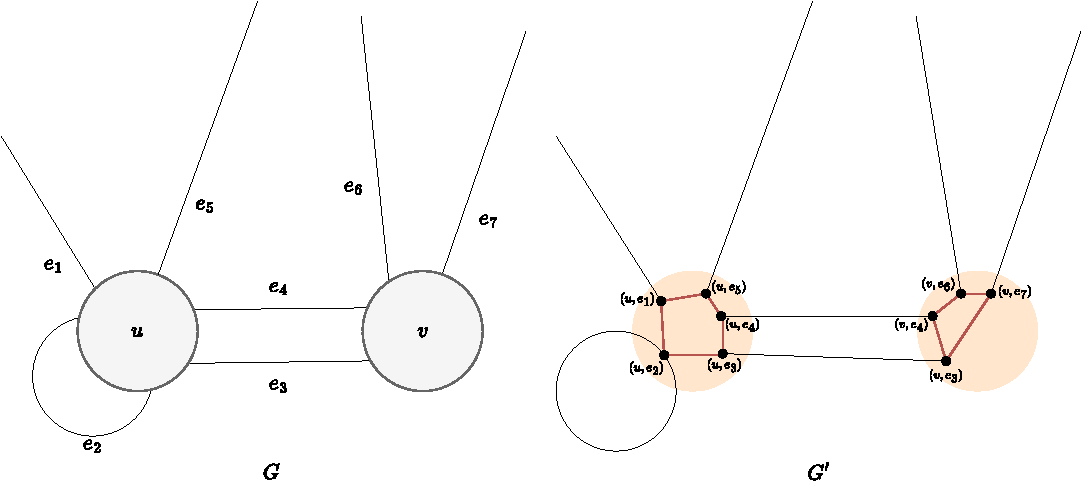
\includegraphics[width=\textwidth]{images/degree_reduction.pdf}
  \caption{次数削減変換の例. 橙色の内部の頂点集合がクラウドであり, クラウド内の辺は\cref{thm:construction-of-expander-graph}によって構成されるが, ここでは図の簡単のため$X_d$を長さ$d$の閉路としている. $G'$における黒い辺の制約は対応する元のグラフの辺と同一の制約とし, クラウド内の赤辺の制約は等式制約とする.}
  \label{fig:degree-reduction}
\end{figure}

元のグラフの各頂点$u\in V$に対し, 
\[[u]=\qty{ (u,e) \in \{u\}\times E \colon e=\{u,v\} \text{ for some } v\in V }\]
を(この証明のローカルな用語として)\emph{$u$-クラウド}と呼ぶことにする.
新しい頂点集合$V'$は$V'=\bigcup_{u\in V} [u]$である.
すなわち, $u$をそれに接続する辺の本数(自己ループは1個分としてカウント)だけコピーして得られる集合が$[u]$である.

次に辺集合$E'$を以下のように構成する.
まず, $(X_n)_{n\in\Nat}$を\cref{thm:construction-of-expander-graph}によって構成される$n$頂点$d_0$-正則$\lambda$-エクスパンダーの族とする.
元のグラフの各頂点$u\in V$に対し, $d=\abs{[u]}$としたとき, 頂点集合$[u]$上で$X_d$と同型なグラフを構成し, それを$([u],E_u)$とする.
このとき, 各$u$-クラウド内部の辺集合$E_{\mathrm{inner}}$は
\begin{align*}
  E_{\mathrm{inner}} = \bigcup_{u\in V} E_u
\end{align*}
とする.
次に異なるクラウド間を繋ぐ辺集合$E_{\mathrm{outer}}$を
\begin{align*}
  E_{\mathrm{outer}} = \qty{\qty{ (u,e), (v,e) } \colon e\notin [u]\cap[v]}
\end{align*}
とする.
このとき, グラフ$G'$の辺集合$E'$は
\begin{align*}
  E' = E_{\mathrm{inner}} \cup E_{\mathrm{outer}}
\end{align*}
となる.

次に各辺$e'\in E'$の制約$c'_{e'}$を以下のように定める:
\begin{itemize}
\item 辺$e'\in E_{\mathrm{outer}}$がクラウド間をつなぐ辺ならば, その制約は対応する元の辺$e$の制約と同じとする.
すなわち, $e'=\qty{ (u,e), (v,e) }$ならば, $c'_{e'}=c_e$である.
\item 辺$e'\in E_{\mathrm{inner}}$がクラウド内部の辺ならば, その制約を$c'_{e'}=\{(\sigma,\sigma)\colon \sigma\in\Sigma\}$, すなわち等式制約とする.
\end{itemize}

このようにして得られる制約グラフ$G'=\ip{(V',E'),\Sigma,\calC'}$が補題の主張を全て満たすことを確認する.
まず, $G'$は$(d_0+1)$-正則である.
実際, $G'$の各頂点$(u,e)\in V'$に接続する辺は, クラウド内の辺が$d_0$本, クラウド間の辺が$1$本である.
また, $G$から$G'$を構成する際に新たに追加する辺は$E_{\mathrm{inner}}$のみであり, これは高々$\sum_{u\in V}\frac{d_0\deg_G(u)}{2} \le d_0\abs{E}$本である (ここで\cref{eq:hand_shake_multigraph}を用いた).
従って
\begin{align}
  \abs{E'} = \abs{E_{\mathrm{inner}}} + \abs{E_{\mathrm{outer}}} \le \qty(d_0+1)\abs{E} \label{eq:bound_of_E'}
\end{align}
を満たす.
また, $V'$の要素数は次数の総和に等しいため, $\abs{V'}\le 2\abs{E}$を満たす.
次に, $\UNSAT(G)=0$ならば$\UNSAT(G')=0$である.
実際, 元の制約グラフの全ての制約を満たす割り当て$a\colon V\to\Sigma$に対し, $G'$の割り当て$a'\colon V'\to\Sigma$を
\begin{align*}
  a'(u,e) = a(u)
\end{align*}
と定めると, $a'$は$G'$の制約を満たす (同一クラウド内の頂点には全て同じ値が割り当てられるため, クラウド内の辺の制約は全て満たされ, クラウド間の辺に対応する制約は$a$の取り方により全て満たされることがわかる).

最後の主張, すなわち$\UNSAT(G') \ge c'\cdot \UNSAT(G)$となる定数$c'>0$が存在すること示す.
定数$c'>0$を
\begin{align}
  c' = \min\qty{\frac{(1-\lambda_0)d_0}{8(d_0+1)}, \frac{1}{2(d_0+1)}} \label{eq:c_of_degree_reduction}
\end{align}
と定める.
$\UNSAT(a';G')=\UNSAT(G')$を満たす割り当て$a'\colon V'\to\Sigma$を任意に取る.
この割り当て$a'$に対し, 元のグラフ$G$の割り当て$a\colon V\to\Sigma$を
\begin{align*}
  a(u) = \Maj((a'(u,e))_{(u,e) \in [u]})
\end{align*}
と定める. ここで$\Maj(\cdot)$は多数決関数であり,
タイは任意に選ぶとする.
例えば$\Maj(1,2,2)=2$, $\Maj(1,2,3,3)=3$, $\Maj(1,2,2,3,3)=2$である ($\Maj(1,2,2,3,3)=3$としても良いが, ここでは便宜上小さい方の数字を採用している).

以降, 割り当て$a'\colon V'\to\Sigma$に対し, 頂点$(u,e)\in V'$への割り当て$a'(u,e)$を頂点$(u,e)$の\emph{意見}と呼ぶこととする.
同様に, 割り当て$a\colon V\to\Sigma$に対し, 頂点$u\in V$への割り当て$a(u)$を頂点$u$の意見と呼ぶこととする.
直感的には頂点$u$の意見は対応する$u$-クラウド内の頂点の意見の多数決である.


辺集合$F\subseteq E$を割り当て$a$によって充足されない辺の集合, すなわち
\begin{align*}
  F = \qty{ e=\{u,v\}\in E \colon (a(u),a(v)) \not\in c_e}
\end{align*}
と定義する.
ここで$\calC = (c_e)_{e\in E}$は元の制約グラフ$G$の制約である.
同様に, $F'\subseteq E'$を割り当て$a'$によって充足されない辺の集合とする.
このとき$\UNSAT(a;G) = \frac{|F|}{|E|}$および$\UNSAT((a';G') = \frac{|F'|}{|E'|}$である.
頂点部分集合$S\subseteq V'$を$a$の多数決で選ばれなかった意見を持つ頂点の集合, すなわち
\begin{align*}
  S = \qty{ (u,e) \in V' \colon a(u) \ne a'(u,e)}
\end{align*}
と定義し, 各$v\in V$に対し$S^v = S\cap [v]$とし, 各$\sigma\in \Sigma$に対し$S^v_\sigma = \qty{ (u,e)\in S^v \colon a'(u,e)=\sigma }$とする (\cref{fig:majority-degree-reduction}).
なお, $\sigma\in\Sigma$が多数決の意見 (すなわち$\sigma=a(v)$)のとき, $S^v_\sigma=\emptyset$とする.

\begin{figure}[ht]
  \centering
  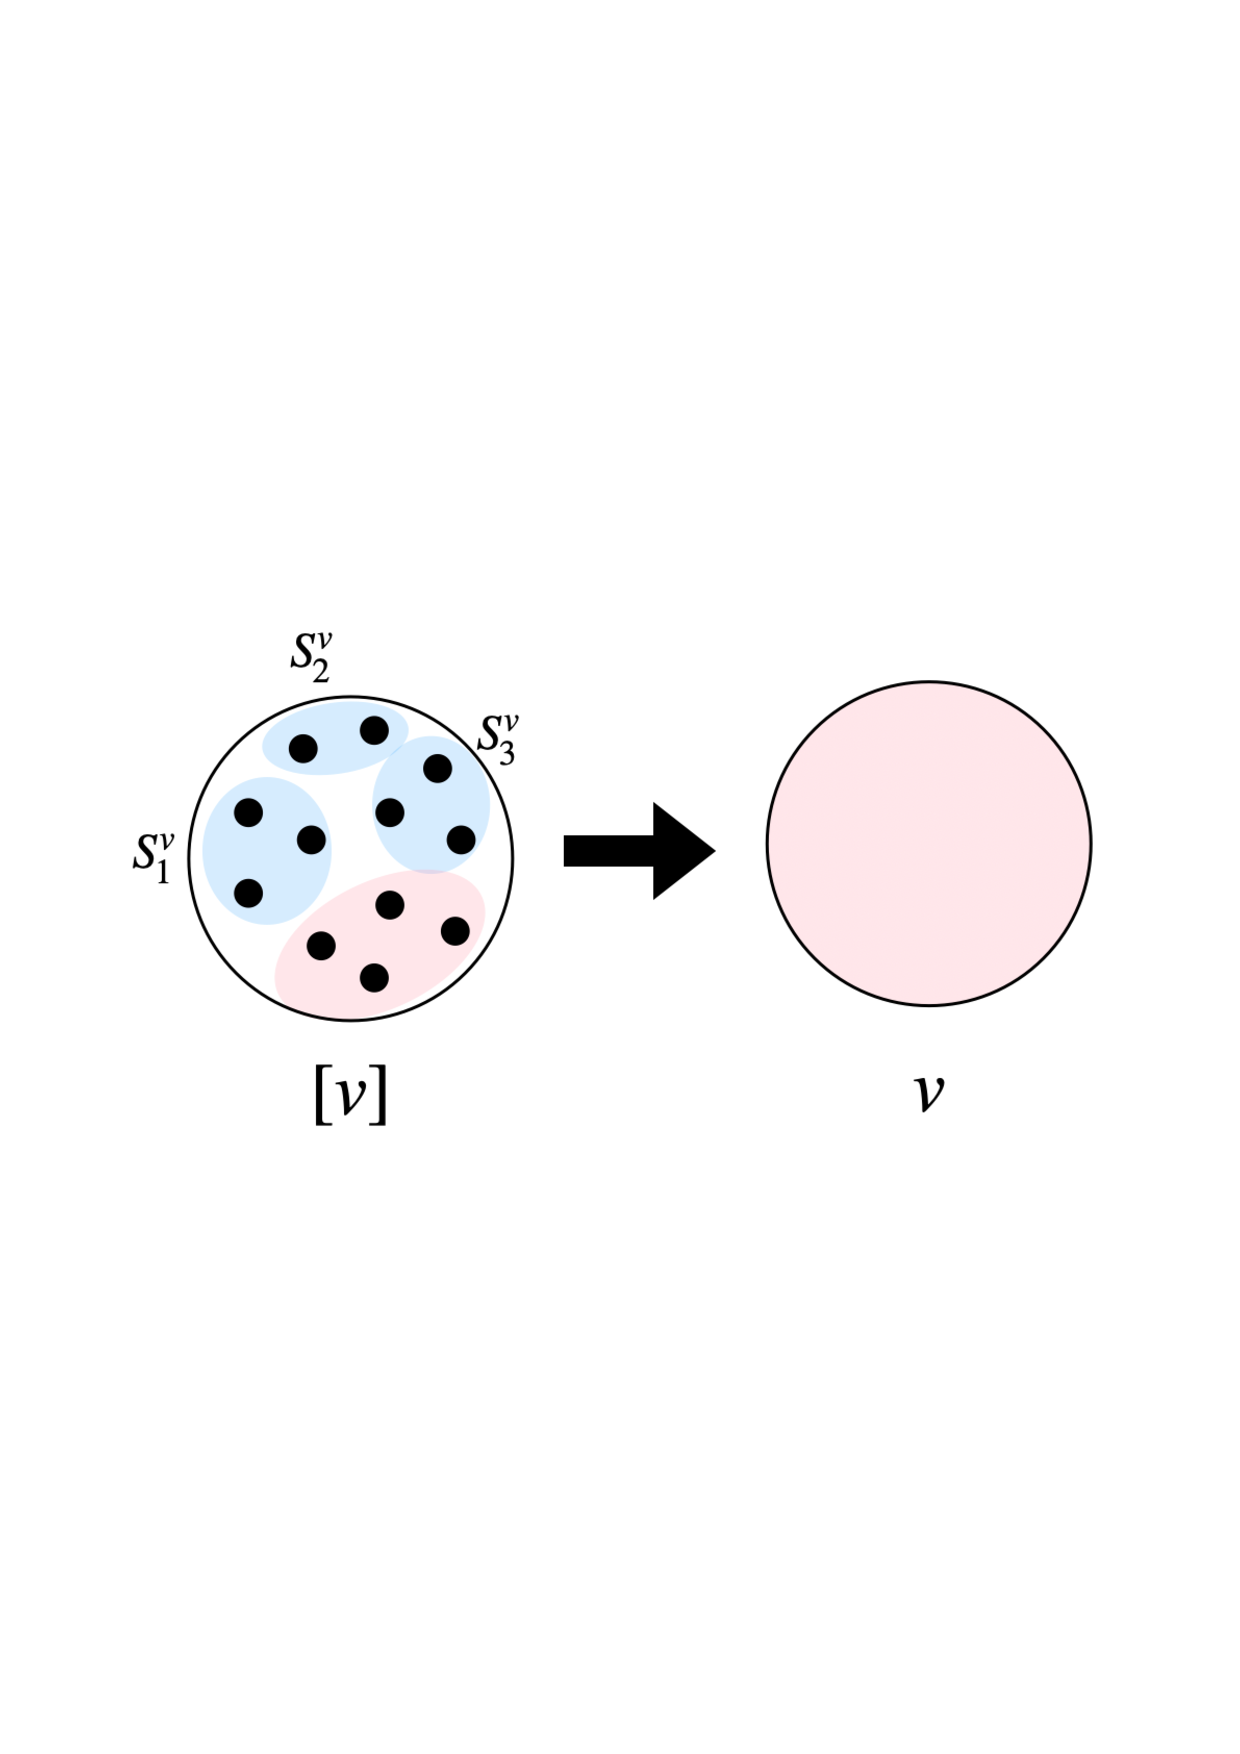
\includegraphics[width=\textwidth]{images/majority_degree_reduction.pdf}
  \caption{多数決によって選ばれなかった$v$-クラウド内の頂点の集合を$S_v\subseteq [v]$とする. \label{fig:majority-degree-reduction}}
\end{figure}

以下の二つのケースを考える:

\paragraph*{ケース1. $\abs{S} \ge \frac{\UNSAT(a;G)}{2}\abs{E}$の場合.}

各頂点$v\in V$と多数決によって選ばれなかった意見$\sigma\in\Sigma \setminus \{a(v)\}$に対し$\abs{S^v_\sigma} \le \frac{\abs{[v]}}{2}$である
(そうでなければ意見$\sigma$が多数決によって選ばれなかったことに矛盾する).
ここで$v$-クラウド内部のグラフは$d_0$-正則$\lambda_0$-エクスパンダーであるため, その頂点部分集合$S^v_\sigma\subseteq[v]$に対するエクスパンダー混交補題(\cref{lem:expander-mixing-lemma})より,
\begin{align*}
  W(S^v_\sigma, [v]\setminus S^v_\sigma) \ge (1-\lambda_0)\cdot \frac{d_0\abs{S^v_\sigma}}{2}
\end{align*}
となる. ここで$W(S,T)$は$v$-クラウド内部のグラフ$([v],E_v)$の辺であって$S$と$T$の間をまたがる辺の本数である.
ここで$S^v_\sigma$と$[v]\setminus S^v_\sigma$をまたがる全ての辺の両端点の意見は異なるため, $a'$はこれらの辺を充足しない. よってこれらの辺は全て$F'$に含まれる.
従って
\begin{align*}
  \abs{F'} &\ge \frac{1}{2}\sum_{v,\sigma} W(S^v_\sigma, [v]\setminus S^v_\sigma) \\
  &\ge \frac{(1-\lambda_0)d_0}{4}\sum_{v,\sigma} \abs{S^v_\sigma} \\
  &= \frac{(1-\lambda_0)d_0}{4}\abs{S} \\
  &\ge \frac{(1-\lambda_0)d_0}{8}\UNSAT(a;G)\cdot \abs{E}  & & \because \text{ケース1の仮定} \\
  &\ge \frac{(1-\lambda_0)d_0}{8(d_0+1)}\UNSAT(a;G)\cdot \abs{E'}. & & \because\text{\cref{eq:bound_of_E'}}
\end{align*}
特にこれから$\UNSAT(a';G') = \frac{\abs{F'}}{\abs{E'}}\ge \frac{(1-\lambda_0)d_0}{8(d_0+1)}\cdot\UNSAT(a;G)$が成り立つ.

\paragraph*{ケース2. $\abs{S} < \frac{\UNSAT(a;G)}{2}\abs{E}$の場合.}
任意の辺$e = \{u,v\} \in F$に対して, それに対応する$G'$の辺$e' = \{(u,e),(v,e)\}$を考える.
\begin{itemize}
\item もしも$a(u)=a'(u,e)$かつ$a(v)=a'(v,e)$が成り立つならば, $e'$と$e$は同じ制約を持ち, $e\in F$であることから$e'\in F'$である.
\item そうでない, すなわち$a(u)\ne a'(u,e)$または$a(v)\ne a'(v,e)$が成り立つならば, $(u,e)$と$(v,e)$のうち少なくとも一方はその意見が多数決として選ばれない, すなわち$(u,e)\in S$または$(v,e)\in S$が成り立つ.
\end{itemize}
以上より$\abs{F} \le \abs{F'} + \abs{S}$が成り立つので
\begin{align*}
  \abs{F'} &\ge \abs{F} - \abs{S} \\
  &\ge \abs{E}\UNSAT(a;G) - \frac{\UNSAT(a;G)}{2}\abs{E} & & \because \text{ケース2の仮定}\\
  &= \frac{\UNSAT(a;G)}{2}\abs{E} \\
  &\ge \frac{\UNSAT(a;G)}{2(d_0+1)}\abs{E'} & & \because\text{\cref{eq:bound_of_E'}}
\end{align*}
となり, これから
\begin{align*}
  \UNSAT(a';G') = \frac{\abs{F'}}{\abs{E'}} \ge \frac{1}{2(d_0+1)}\cdot \UNSAT(a;G)
\end{align*}
が成り立つ.

ケース1,2より, \cref{eq:c_of_degree_reduction}で定まる定数$c'>0$に対して$\UNSAT(a';G') \ge c'\cdot \UNSAT(a;G) \ge c'\cdot \UNSAT(G)$が成り立つ.
\end{proof}

\subsection{エクスパンダー化}

次に, 与えられた正則な制約グラフをエクスパンダーグラフに変換する補題を示す.

\begin{lemma}{エクスパンダー化補題}{expanderization}
ある定数$\lambda<1,d,d_0\in\Nat$および次を満たす多項式時間アルゴリズム$A$が存在する:
アルゴリズム$A$は入力として$d$-正則な制約グラフ$G = \ip{ (V,E), \Sigma, \calC }$
を受け取り, $(d+d_0+1)$-正則で全頂点が自己ループを持ち, さらに$\lambda$-エクスパンダーである制約グラフ $G' = \ip{ (V, E'), \Sigma, \calC' }$ を出力する.
さらに, この制約グラフ$G'$は$\UNSAT(G') = \frac{d}{d+d_0+1}\UNSAT(G)$を満たす.
\end{lemma}

\begin{proof}
入力として与えられた制約グラフを$G=\ip{(V,E),\Sigma,\calC}$とする.
変換は以下のようにして行われる:
\begin{enumerate}
\item まず, \cref{thm:construction-of-expander-graph}を用いて頂点集合$V$上$d_0$-正則$\lambda_0$-エクスパンダーグラフを構成し, その辺集合を$E$に追加する (この際多重辺も許す).
\item 次に, 各頂点に自己ループを付与する.
\item ステップ1,2で追加した辺$e$に対応する制約$c'_e$を自明な制約$c'_e=\Sigma^2$とする.
\end{enumerate}
このようにして得られる制約グラフを$G'=\ip{(V',E'),\Sigma,\calC'}$とする.
元の制約グラフ$G$が$d$-正則であることから, $G'$は$(d+d_0+1)$-正則である (自己ループの次数への寄与は$1$であることに注意).
また, ステップ2より$G'$は全頂点が自己ループを持つ.

次に$\UNSAT(G')=\frac{d}{d+d_0+1}\UNSAT(G)$を示す.
任意の割り当て$a\colon V \to \Sigma$に対し, 
ステップ1,2で追加した辺に対応する制約は常に充足されるため, 両者が充足\emph{しない}制約の個数は一致する.
すなわち$\abs{E}\UNSAT(a;G) = \abs{E'}\UNSAT(a;G')$が成り立つので
\begin{align*}
  \UNSAT(G') = \min_{a}\UNSAT(a;G') = \frac{\abs{E}}{\abs{E'}}\min_a \UNSAT(a;G) = \frac{d}{d+d_0+1}\UNSAT(G)
\end{align*}
が成り立つ.

最後に$G'$が$\lambda:=\frac{d}{d+d_0+1}+\frac{\lambda_0(d_0+1)}{d+d_0+1}$に対し$\lambda$-エクスパンダーであることを示す.
元のグラフ$G$の遷移確率行列を$P\in[0,1]^{V\times V}$とし,
ステップ1,2で追加した辺からなるグラフを$G_0$とし, その遷移確率行列を$P_0\in[0,1]^{V\times V}$とする.
また, 最終的に得られるグラフ$G'$の遷移確率行列を$P'\in[0,1]^{V\times V}$とする.
元のグラフ$G$は$d$-正則, 追加したグラフ$G_0$は$(d_0+1)$-正則であるため
\begin{align*}
  P' = \frac{d}{d+d_0+1}P + \frac{d_0+1}{d+d_0+1}P_0
\end{align*}
となる.
さらに$P_0$は$\lambda_0$-エクスパンダーであるため, 全成分$1$のベクトル$\allone$と直交する任意のベクトル$x\in \Real^V$に対し
\begin{align*}
  x^\top P' x &= \frac{d}{d+d_0+1}x^\top P x + \frac{d_0+1}{d+d_0+1}x^\top P_0 x \\
  &\ge \frac{d}{d+d_0+1}\norm{x}^2 + \frac{d_0+1}{d+d_0+1}\lambda_0\norm{x}^2 & & \because\text{$P_0$のエクスパンダー性}\\
  &\le \qty( \frac{d}{d+d_0+1} + \frac{\lambda_0(d_0+1)}{d+d_0+1} )\norm{x}^2
\end{align*}
より, $\lambda(P')\le \frac{d}{d+d_0+1} + \frac{\lambda_0(d_0+1)}{d+d_0+1}$が成り立つ.
\end{proof}

これにより\cref{lem:constant-degree-expanderization}を示す準備が整った.
\begin{proof}[\cref{lem:constant-degree-expanderization}の証明]

与えられた制約グラフ$G$に対し, まず$G$を入力として\cref{lem:degree-reduction}のアルゴリズムを実行し, その出力を$G_1$とする.
この制約グラフ$G_1$は\cref{lem:degree-reduction}の主張より, $d$-正則である.
次に, $G_1$を入力として\cref{lem:expanderization}のアルゴリズムを実行し, その出力を最終的な出力$G$とする.
この制約グラフ$G'$は\cref{lem:expanderization}の主張より, 全頂点が自己ループを持ち, $(d+d_0+1)$-正則かつ$\lambda$-エクスパンダーである.
また, この一連の変換によって$\size(G')$は$\size(G)$の定数倍にしかならない.

最後に$\UNSAT$の値を考える.
元の制約グラフ$G$が$\UNSAT(G)=0$ならば, \cref{lem:degree-reduction,lem:expanderization}より
$\UNSAT(G') = \frac{d}{d+d_0+1}\UNSAT(G_1) = 0$を得る.
一方で
\begin{align*}
  \UNSAT(G') = \frac{d}{d+d_0+1}\UNSAT(G_1) \ge \frac{d}{d+d_0+1}\cdot c'\cdot\UNSAT(G).
\end{align*}
すなわち$\beta = \frac{d}{d+d_0+1}\cdot c'$に対して主張が成り立つことが示された.
\end{proof}



